\chapter{Konzepte}
\label{sec:konzepte}

In diesem Kapitel werden Konzepte beschrieben, die möglichst abstrakt gehalten sind. Entwickler eines Online-Multiplayer Spiels sollen anhand von diesen Konzepten eine Hilfestellung bekommen, um einen roten Faden in ihrer Entwicklung verfolgen zu können.

Bevor eines dieser Konzepte angewandt werden kann, müssen folgende Voraussetzungen erfüllt sein:

1. Das grundsätzliche Spielkonzept wurde erarbeitet und steht fest.

2. Anhand von dem festgelegten Spielkonzept kann abgeschätzt werden, ob sich für das Spiel eine Client / Server oder eine Client / Host Architektur eignet.

Sollte das Team bzw. der Solo-Entwickler zum Entschluss gekommen sein dass sich ein Client / Server Modell am besten für den spezifischen Use-Case eignet, so müssen vorab Vorkehrungen getroffen werden, um die Hardware-Ressourcen für den späteren Server-Runner sicher zu stellen. Die Grundvoraussetzung ist jedoch ein aus dem Internet erreichbarer PC mit einer festen IP-Adresse.

\begin{quote}
	Distribution concepts
	
	"There is not much we can do about the aforementioned resource limitations. Therefore, the problems of distributed interactive systems should be tackled on a higher level, which means choosing architectures for communication, data, and control. Still, sometimes the architecture alone cannot rid the system of resource limitations, and compensatory techniques are needed to relax the requirements." \cite{Smed.2002}
\end{quote}


Nun gilt es einen passenden Technologie-Stack zu finden. Hier gibt es keine Klare Empfehlung, jedoch können die in diesem Kapitel beschriebenen Konzepte als Entscheidungshilfe dienen. Auf dem offenen Markt existieren bereits Frameworks \& Game Engines, die Manche dieser Konzepte bereits implementiert haben und als Libraries für Entwickler bereitstellen.

\cite{MFatihMAR.2021}


\section{API für Matchmaking \& Server Runner}

Bei diesem Konzept muss eine API entworfen werden, welche unabhängig von einem existierenden Client oder Serverprozess arbeitet. Diese API hat 2 grundsätzliche Aufgaben. 

Matchmaking:

Die API muss einen Algorithmus implementieren, welcher mehrere Spieler zu einer Spiel-Session zusammenführt. Mögliche Matchmaking Konzepte sind bereits im Hintergrund-Kapitel beschrieben. Die Matchnaking API verwaltet als eine Liste an aktiven Serverprozessen sowie die Information, wie man sich zu ihnen verbindet. In der Regel wird pro Serverprozess ein Netzwerk-Port an der Server-Maschine reserviert, auf denen sich dann N Spieler verbinden können.

Je nach Spielkonzept können hunderte, tausende Serverprozesse existieren, welche jeweils nur eine vergleichsweise geringe Anzahl (1-20) an Spieler verwalten. Spielkonzepte, welche viele Spieler (200-1000) innerhalb eines einzigen Serverprozesses voraussetzten, erzeugen dagegen zwar quantitativ weniger Serverprozesse, diese neigen aber in der Regel schnell zu Überlastung. Neben der Umsetzung von Interest Management und einer schlanken Architektur für möglichst wenig Network-Traffic kann aber auch die Matchmaking API Abhilfe schaffen, bspw. durch "Umverlegung" von Spielern auf andere oder neue Serverprozesse.

Server Runner:

Neben dem Matchmaking ist die API ebenfalls auch zuständig für das Starten und die Überwachung von Serverprozessen.
Ebenfalls können technische Statusinformationen über aktuell laufende Spiel innerhalb eines Serverprozesses von der API verwaltet werden (Bspw. ob es möglich ist einem Server beizutreten, oder wieviele Spieler bereits auf einem Serverprozess spielen)

\begin{figure}
	\centering
	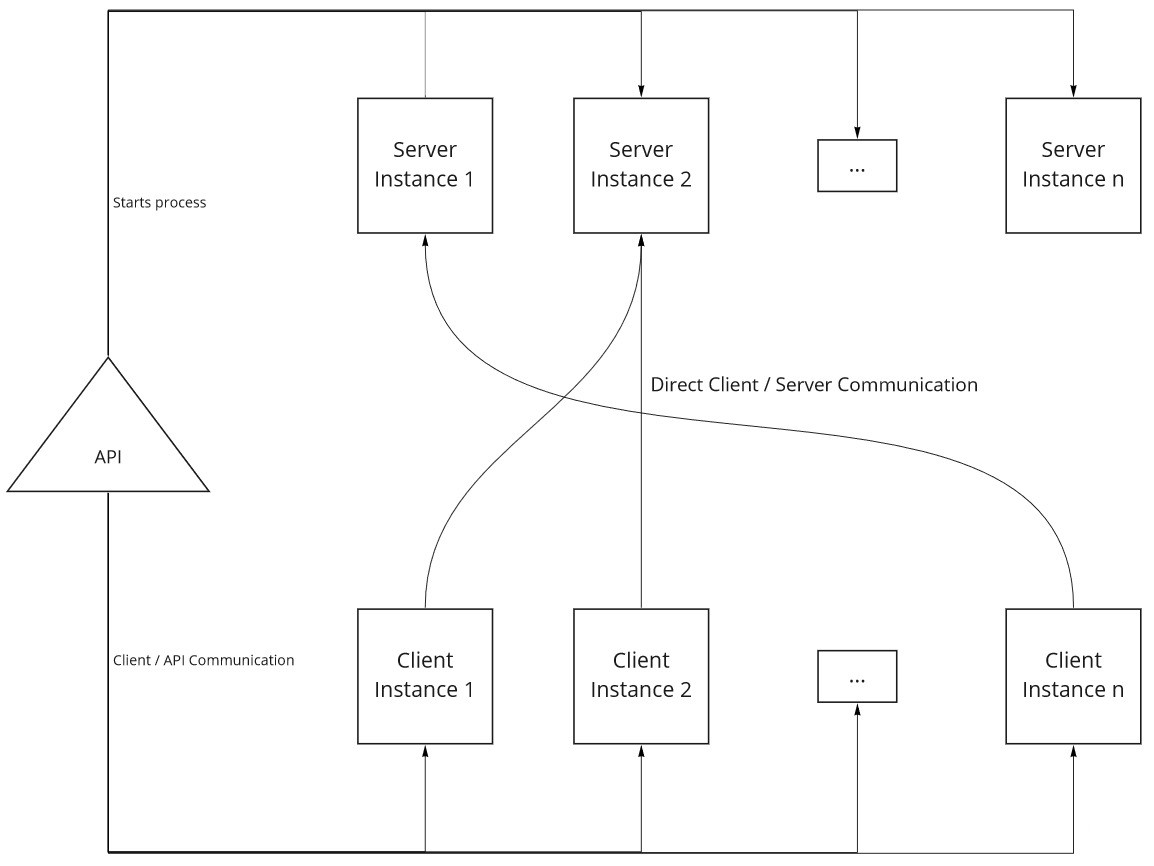
\includegraphics[width=150mm]{images/API_Konzept_Diagramm.jpg}
	\caption[API Konzept Diagramm]{Veranschaulichung des API Konzepts}
	\label{pic:API_Konzept_Diagramm}
\end{figure}


Je nach Use-Case kann das Aufgabenfeld der API um weitere Punkte erweitert werden, hier ein paar Beispiele:
--> Datenbank für Authentifizierung bzw. Kommunikation mit externen SSO-Service Providern \cite{Wikipedia.2021c} 
--> Datenbank für InGame Shop / Kommunikation mit externen Lösungen


\section{Client UI \& Visual Controller}

Das Konzepts des Client UI \& Visual Controllers beschreibt die Art und Weise, wie die Benutzeroberfläche und visuelle Ebene eines Spielers durch Antworten des Servers oder einzelner Spieleraktivitäten manipuliert wird.

\begin{figure}
	\centering
	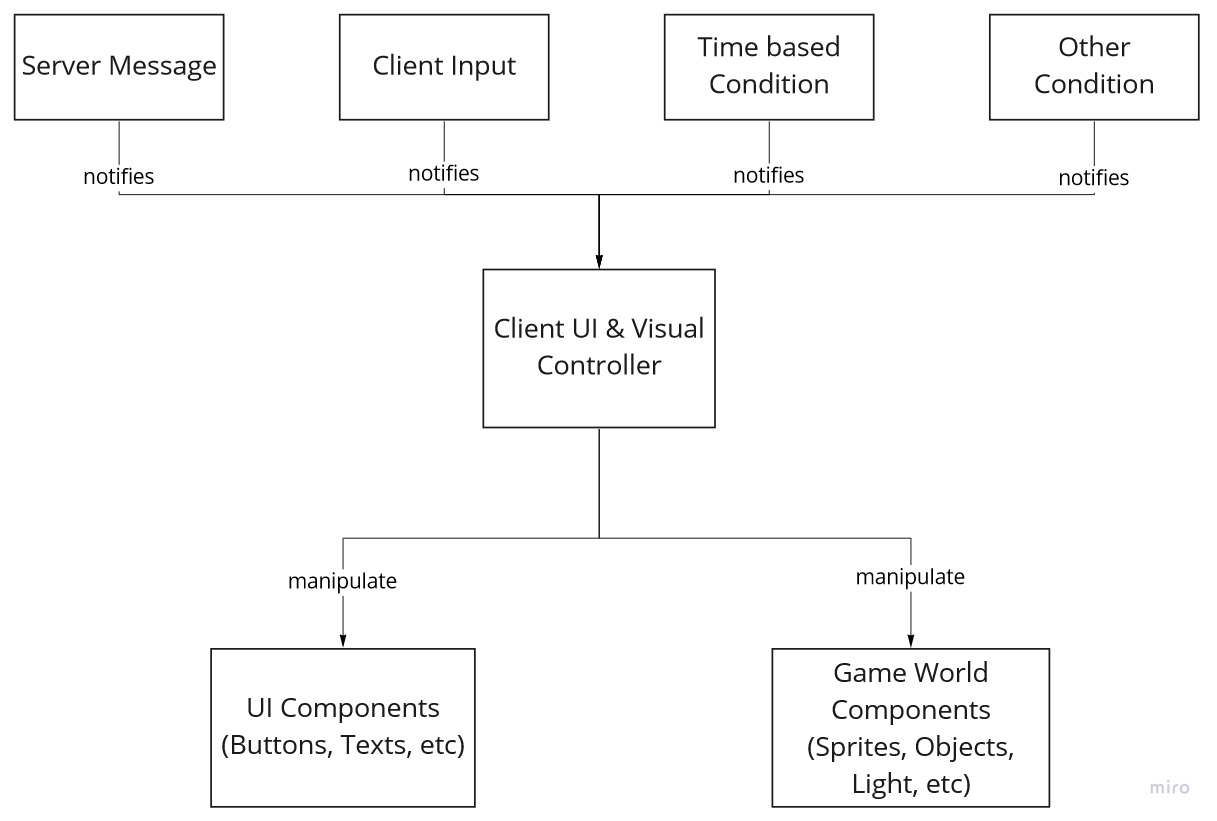
\includegraphics[width=150mm]{images/Client_UI_und_Visual_Konzept.jpg}
	\caption[Client UI \& Visual Controller Diagramm]{Veranschaulichung des Client UI \& Visual Controller Konzepts}
	\label{pic:Client_UI_und_Visual_Konzept}
\end{figure}

Konkret sorgt ein Server-Ereignis, der Input eines Spielers (beispielsweise durch klicken eines Buttons oder einsammeln eines Gegenstands) oder eine andere Bedingung dafür, dass Funktionen innerhalb des Client UI \& Visual Controllers aufgerufen werden. Innerhalb dieser Funktionen werden Komponenten der Benutzeroberfläche wie z.b. Anzeigetexte, Bilder etc. oder Objekte innerhalb der Spielwelt selbst manipuliert.

Wichtig ist, dass Funktionen des Client UI \& Visual Controller erst nach server- oder clientseitigen Überprüfungen ausgeführt werden. Der Controller selbst sollte nur überprüfen, ob die Komponente, welche er manipulieren will überhaupt existiert. Spielrelevante Logik, beispielsweise ob ein Spieler berechtigt ist, bestimmte Aktionen durchzuführen, ist nicht Teil des Client UI \& Visual Controllers.

\section{Client Connection Manager}

Das Konzept Client Connection Manager beschreibt eine Softwarekomponente, welche folgende Aufgaben umsetzen muss:

- Implementierung von clientseitigen Methoden zum Informationsaustausch mit Matchmaking API.
Z.B. stellt die Matchmaking API dem Client über HTTP-Kommunikation Informationen bereit, mit denen sich der Client auf einen speziellen Server verbinden kann (IP + Port). \cite{Wikipedia.2021d} \cite{Wikipedia.2021e}

- Verarbeitung der von Matchmaking API bereitgestellten Informationen. 

Z.B. könnte die Matchmaking API einem Client die Information bereit stellen, dass aus einem bestimmten Grund dem angeforderten Serverbeitritt verweigert wird. Diese Information muss der Client Connection Manager "Zwischenspeichern" und verwalten.

- Aufruf von Methoden eines Client UI Controllers.

Z.B. Die soeben erlangte Information über den verweigerten Serverbeitritt muss nun dem Nutzer dargestellt werden, hierfür ruft der Client Connection Manager Funktionen auf, welche ein Client UI Controller implementiert hat.)

- Ausführen von Handler-Funktionen und Auslösen von Callbacks für clientseitige Konsequenzen bei Netzwerkabbruch, manuellem Verlassen einer Server-Session oder sonstigen Abbruchgründen, welche dazu führen, dass eine Online-Spielsession verlassen wird.

Z.B. Wird die notwendige Verbindung zum Internet während des Spiels unterbrochen. Der Client Connection Manager löst Callbacks aus, welche im Client UI \& Visual Controller implementiert sind. Diese Sorgen dafür, dass der Spieler zurück ins Hauptmenü geleitet wird, in dem eine Fehlermeldung dargestellt wird, welche erklärt warum das Spiel abgebrochen ist.

\begin{figure}
	\centering
	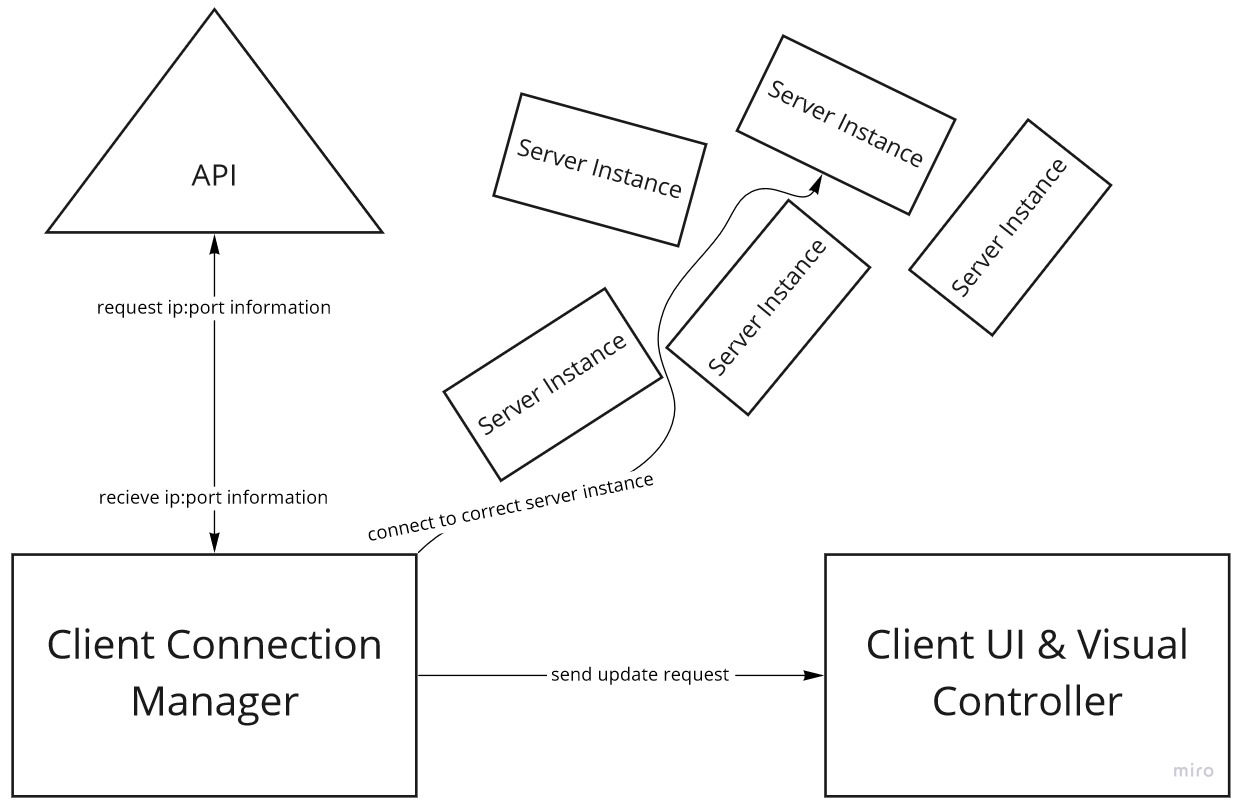
\includegraphics[width=150mm]{images/Client_Connection_Manager.jpg}
	\caption[Client Connection Manager Diagramm]{Veranschaulichung des Client Connection Manager Konzepts}
	\label{pic:Client_Connection_Manager}
\end{figure}



\section{Serverside Client Management}

// TODO Add Content

\section{Prepare-Game-Manager}

// TODO Add Content

\section{Progress Manager / State Manager}

// TODO Add Content

\section{Spawn Manager}

// TODO Add Content

\section{Entwicklung sonstiger Server Logik}

(Hier vielleicht noch ein paar Konzepte rausarbeiten)

\section{Entwicklung sonstiger Client Logik}

(Hier vielleicht noch ein paar Konzepte rausarbeiten)

\section{Studienkonzept}

// TODO Add Content

Wie können diese Konzepte auf Hand und Fuß überprüft werden?

